\documentclass[a4paper]{FedericoIIswedoc}
\usepackage{./Custom/frontpage}
\usepackage{./Custom/blankpage}
\usepackage{./Custom/glossary}

\fpthesistitle{BugBoard26}
\fpthesissubtitle{Documentazione del progetto di Ingegneria del Software}
\fpfirstauthor{Mario Lombardo}{N86004029}
\fpsecondauthor{Giuseppe Pollio}{N86004953}
\fpthirdauthor{Antonio Paudice}{N86004566}
\fpprofessors{Porfiro Tramontana \\ Breve Bernardo}

\fpschool{Università degli Studi di Napoli Federico II}
\fpdegree{Classe di Laurea in Scienze e Tecnologie Informatiche L-31}

\fpthesisdate{Anno Accademico 2025/2026}

\fpschoollogo{./Assets/Federico_II_University_Logo_White.png}
\fpbackgroundimage{./Assets/cover.png}


\begin{document}
	\makefrontpage
	\blankpage
	
	% Numerazione romana per le pagine iniziali
	\pagenumbering{roman}
	
	\tableofcontents
	\newpage
	
	\listoffigures
	\addchapterlike{Lista delle Figure}
	\newpage
	
	\listoftables
	\addchapterlike{Lista delle Tabelle}
	\newpage
	
	
	
\glossaryentry{API}{Application Programming Interface - Interfaccia di programmazione delle applicazioni}
\glossaryentry{UML}{Unified Modeling Language - Linguaggio di modellazione unificato utilizzato per la specifica, visualizzazione e documentazione dei sistemi software}
\glossaryentry{Framework}{Struttura di supporto su cui un software può essere organizzato e progettato}
\glossaryentry{Repository}{Archivio centralizzato dove vengono memorizzati e gestiti i dati del progetto}



	\printglossary
	\addchapterlike{Glossario}
	\blankpage
	\cleardoublepage
	
	
	\pagenumbering{arabic}
	
	
\chapter{Introduzione}
Il progetto \textbf{BugBoard26} ha come obiettivo la realizzazione di una piattaforma per la \textbf{gestione collaborativa di issue} in progetti software.
Il sistema consente a team di sviluppo di \textbf{segnalare, assegnare, monitorare e risolvere problematiche} legate al ciclo di vita di un progetto. 
\\\\
Il documento illustra l’analisi e la specifica dei requisiti funzionali e non funzionali, la modellazione dei casi d’uso e la prototipazione delle interfacce.

	\chapter{Descrizione Requisiti}
I requisiti del sistema definiscono ciò che l’applicazione deve fare e come deve operare.\\
I \textbf{Requisiti Di Sistema} descrivono le funzionalità principali e le caratteristiche tecniche necessarie al corretto funzionamento del software, quali autenticazione e gestione dei progetti/issues.\newline
I \textbf{Requisiti Non-Funzionali} specificano le qualità del sistema, concentrandosi su come deve operare. Include aspetti come sicurezza, usabilità e performance, garantendone efficienza, stabilità e affidabilità.
\section{Requisiti di sistema}
\begin{itemize} %----LISTA REQUISITI-----%
	
	\item \textbf{Gestione Autenticazione:} Il sistema deve consentire il login a utenti tramite email e password, distinguendoli tra utenti \textit{Normali} e \textit{Admin}.
	
	\item \textbf{Gestione Progetti:} Schermata iniziale dov'è possibile visualizzare e cercare tutti i progetti a cui l'utente lavora, con informazioni annesse come il numero di \textit{issues} aperte per progetto e il numero di membri che ci partecipano.\\
	Nel caso dell'\textit{admin}, dev'essere possibile anche gestire progetti già esistenti o crearne di nuovi.
	
	
	\item \textbf{Creazione Issues:} Gli \textit{admin} devono poter creare nuove \textit{issues}, specificando tipo, priorità e una breve descrizione, mentre gli utenti normali possono segnalare nuove \textit{issues} agli admin; opzionalmente si possono anche inserire un'immagine e uno stato.
	
	\item \textbf{Assegnazione Issues:} Gli \textit{admin} devono poter assegnare \textit{issues} a membri del progetto, notificando gli utenti interessati.
	
	\item \textbf{Gestione stati:} Il sistema deve consentire il cambiamento degli stati delle issueus, sia dagli \textit{Admin} sia dagli utenti a cui è stata assegnata un issue.
	
	\item \textbf{Filtraggio Issues:} L’utente deve poter filtrare le issue per nome, tipo (Bug, Feature, Question, Documentation), stato (Aperta, In Progress, Risolta, Chiusa), priorità (Bassa, Media, Alta, Critica) o in base al tempo di creazione.
	
	\item \textbf{Archiviazione Issues:} L'\textit{admin} dev'essere in grado di archiviare \textit{issues} risolte, in modo tale che non siano più visibili nella lista principale ma rimangano consultabili.
	
	\item \textbf{Commenti e aggiornamenti:} Ogni Issue deve poter includere una sezione commenti/aggiornamenti, visibile a tutti i membri del progetto .
	
	\item \textbf{Esportazione dati:} Il sistema dev'essere in grado di consentire l'esportazione dati in vari formati, quali CVS, PDF o Excel.
	
	\item \textbf{Modalità Read-Only:} Il sistema deve permettere la creazione di utenti in sola lettura per esterni al team di sviluppo, che consente di visualizzare \textit{issues}, progetti e commenti senza però permetterne la modifica; La creazione e gestione di questi account è a carico solo degli \textit{Admin} del sistema 
	
\end{itemize}

\section{Requisiti Non-Funzionali}
\begin{itemize}
	\item \textbf{Sicurezza:} Tutti i dati di utenti (progetti, issues) sono accessibili solo 
	previa autenticazione, utilizzando email e password memorizzate in forma cifrata.
	
	\item \textbf{Affidabilità:} Il sistema deve garantire registrazione e conservazione di tutte le modifiche apportate alle \textit{issues} senza perdere informazioni
	
	\item \textbf{Performance:} Il caricamento dei progetti o delle \textit{issues} non deve richiedere tempo eccessivo, con database di dimensioni standard
	
	\item \textbf{Manutenibilità:} Il sistema dev'essere sviluppata in modo modulare per semplificare eventuali manutenzioni e aggiornamenti futuri
	
	\item \textbf{Portabilità:} Dev'essere garantita l'esecuzione del sistema su qualsiasi browser moderno
	
	\item \textbf{Backup e recupero dati:} Devono essere garantiti meccanismi di backup automatico e di esportazione manuale dei dati in vari formati per prevenire perdite accidentali
\end{itemize}

	\chapter{Utenti del sistema}

Per il corretto sviluppo di \textbf{BugBoard26}, è necessario definire quali sono gli utenti che andranno a \textbf{utilizzare il sistema}, e di quali \textbf{competenze} o\textbf{ esigenze} hanno bisogno
\\\\
Il sistema è destinato a team di \textbf{sviluppo software} e, più in generale, a tutte le organizzazioni che necessitano di uno strumento collaborativo per la \textbf{gestione di \textit{issues}, bug e richieste di miglioramento}nei propri progetti informatici.
\\\\
All'interno del sistema sono stati individuati quattro \textit{attori} principali, tutti con accesso a funzionalità diverse:
\begin{enumerate}
	
	\item \textbf{Utente non autenticato:} 
	\begin{itemize}
		\item Ha accesso solo alla schermata di login
		\item Non può accedere a dati a meno che non entra nel proprio account. 
	\end{itemize}
	
	\item \textbf{Utente normale (\textit{User}):} 
	\begin{itemize}
		\item Rappresenta il profilo standard utilizzato dalla maggior parte del team di sviluppo (sviluppatori, tester...)
		\item Può visualizzare i progetti a cui partecipa e le \textit{issues} a lui assegnate.
		\item Può creare nuove \textit{issues} secondo il procedimento già indicato.
		\item Può filtrare e ordinare \textit{issues} in base a vari criteri
		\item Può aggiornare lo stato delle \textit{issues} a lui assegnate
	\end{itemize}
	
	\item \textbf{Utente Admin:} 
	\begin{itemize}
		\item Dispone di privilegi avanzati per gestire al meglio l'intero sistema.
		\item Ha come obiettivo di monitorare e coordinare il lavoro del team.
		\item Ha completa gestione dei progetti, può crearli, eliminarli o modificarli.
		\item Può creare account di qualsiasi tipo, specificandone email, password, e tipo di utenza (Normale/Admin/Read-Only).
		\item Può assegnare \textit{issues} a membri del team e contrassegnare eventuali duplicati.
	\end{itemize}
	
	\item \textbf{Utente in sola lettura (Read-Only):}
	\begin{itemize}
		\item Si tratta di un utente esterno al team di sviluppo, come uno stakeholder o un committente.
		\item Gli account di questa categoria possono essere gestiti e creati solo dagli \textit{admin}
		\item Ha lo scopo di monitorare l'andamento del lavoro senza interferire con il lavoro del team
		\item Può visualizzare progetti, \textit{issues} e commenti, senza però modificare o creare nulla
	\end{itemize}
\end{enumerate}
	\chapter{Casi d'uso}
I \textbf{casi d'uso} descrivono \textbf{scenari concreti} di \textbf{interazione attori-sistema}, illustrando come il software risponde alle azioni dell'utente per soddisfare un obiettivo specifico.\\
Hanno il ruolo di far comprendere il \textbf{flusso operativo} dell'intero sistema.

\section{Use-Case diagram completo}
L'immagine comprende un \textbf{diagramma Use-Case} dell'intero sistema, comprendente di tutti gli \textit{Attori} del sistema e degli 8 casi d'uso assegnati.
\begin{figure}[h]
	\centering
	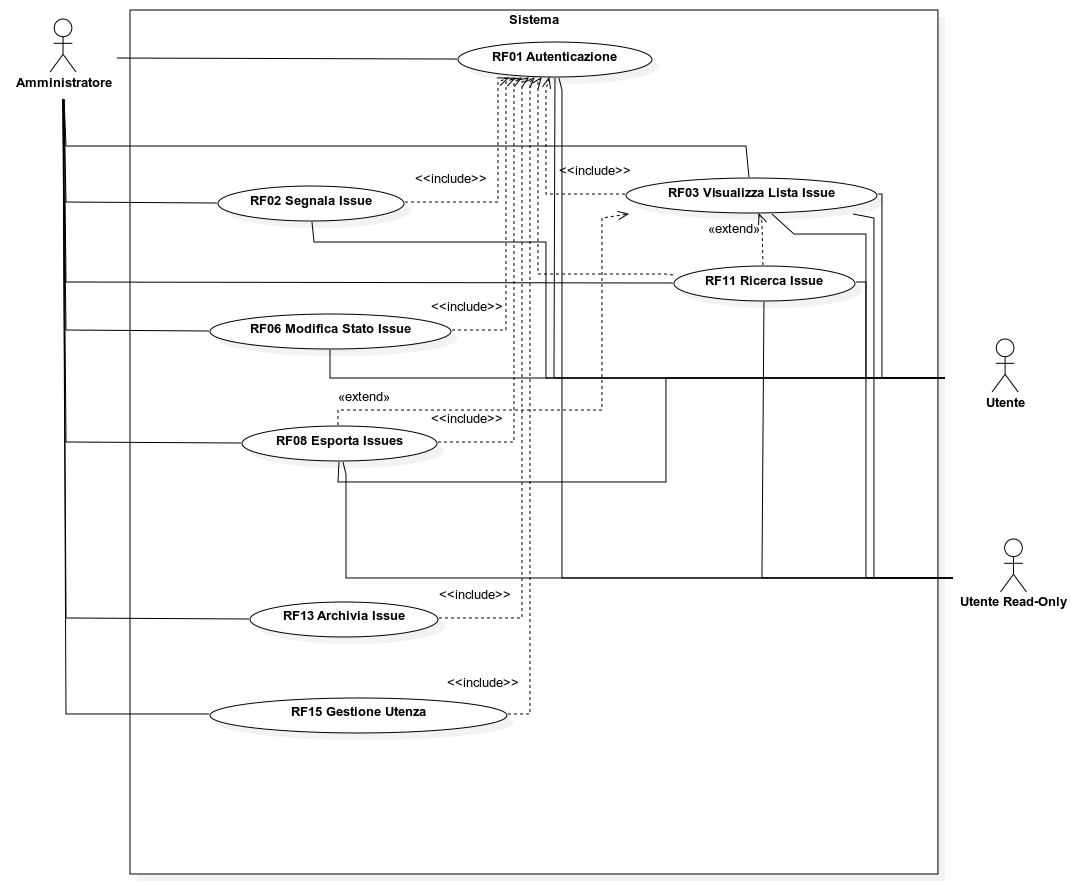
\includegraphics[width=0.7\linewidth]{./Assets/Chapters/use_case.png}
	\caption{Use-Case Completo}
\end{figure}
	
	
\section{Tabella completa Use-Case}
La seguente tabella descrive nel dettaglio i casi d'uso presenti nell'immagine sopra

%---------------------------------------------NON TOCCARE LA TABELLA--------------------------------------------%
\begin{table}[h]
	\caption{Tabella completa Use-Case}
	\begin{tabular}{|c|c|c|c|c|}
		\hline
		ID                           & Titolo                                                                                          & Attori Coinvolti                                                 & Scopo                                                                                                                & Relazioni                                                                                                                                                            \\ \hline
		\rowcolor[HTML]{C8C3BC} 
		UC01                         & \begin{tabular}[c]{@{}c@{}}Autenticazione\\ (RF01)\end{tabular}                                 & \begin{tabular}[c]{@{}c@{}}User\\ Admin\\ Read-only\end{tabular} & \begin{tabular}[c]{@{}c@{}}Accedere al sistema\\ con email e password\end{tabular}                                   & -                                                                                                                                                                    \\ \hline
		UC02                         & \begin{tabular}[c]{@{}c@{}}Segnala Issue\\ (RF02)\end{tabular}                                  & \begin{tabular}[c]{@{}c@{}}User\\ Admin\end{tabular}             & \begin{tabular}[c]{@{}c@{}}Creazione di una nuova\\ issue specificando vari\\ campi\end{tabular}                     & \textless{}\textless{}include\textgreater{}\textgreater RF01                                                                                                         \\ \hline
		\rowcolor[HTML]{C8C3BC} 
		UC03                         & \begin{tabular}[c]{@{}c@{}}Visualizza lista\\ Issue\\ (RF03)\end{tabular}                       & \begin{tabular}[c]{@{}c@{}}User\\ Admin\\ Read-Only\end{tabular} & \begin{tabular}[c]{@{}c@{}}Visualizza l'elenco di \\ issues presenti relative\\ a un progetto specifico\end{tabular} & \textless{}\textless{}include\textgreater{}\textgreater RF01                                                                                                         \\ \hline
		\cellcolor[HTML]{FFFFFF}UC04 & \cellcolor[HTML]{FFFFFF}\begin{tabular}[c]{@{}c@{}}Modifica stato\\ Issue\\ (RF06)\end{tabular} & \begin{tabular}[c]{@{}c@{}}User\\ Admin\end{tabular}             & \begin{tabular}[c]{@{}c@{}}Consente di aggiornare\\ lo stato di una issue,\\ cambiandone i dettagli\end{tabular}     & \textless{}\textless{}include\textgreater{}\textgreater RF01                                                                                                         \\ \hline
		\rowcolor[HTML]{C8C3BC} 
		UC05                         & \begin{tabular}[c]{@{}c@{}}Esporta Issue\\ (RF08)\end{tabular}                                  & \begin{tabular}[c]{@{}c@{}}User\\ Admin\\ Read-Only\end{tabular} & \begin{tabular}[c]{@{}c@{}}Permette di esportare\\ l'elenco di issues in\\ vari formati\end{tabular}                 & \begin{tabular}[c]{@{}c@{}}\textless{}\textless{}include\textgreater{}\textgreater{}RF01\\ \textless{}\textless{}extend\textgreater{}\textgreater{}RF03\end{tabular} \\ \hline
		UC06                         & \begin{tabular}[c]{@{}c@{}}Ricerca Issue\\ (RF11)\end{tabular}                                  & \begin{tabular}[c]{@{}c@{}}User\\ Admin\\ Read-Only\end{tabular} & \begin{tabular}[c]{@{}c@{}}L'utente può cercare una\\ issue utilizzando parole\\ chiave\end{tabular}                 & \begin{tabular}[c]{@{}c@{}}\textless{}\textless{}include\textgreater{}\textgreater{}RF01\\ \textless{}\textless{}extend\textgreater{}\textgreater{}RF03\end{tabular} \\ \hline
		\rowcolor[HTML]{C8C3BC} 
		UC07                         & \begin{tabular}[c]{@{}c@{}}Archivia Issue\\ (RF13)\end{tabular}                                 & Admin                                                            & \begin{tabular}[c]{@{}c@{}}Consente di achiviare le\\ issues, rimuovendola\\ dalla lista principale\end{tabular}     & \textless{}\textless{}include\textgreater{}\textgreater RF01                                                                                                         \\ \hline
		\cellcolor[HTML]{FFFFFF}UC12 & \cellcolor[HTML]{FFFFFF}\begin{tabular}[c]{@{}c@{}}Gestione Utenza\\ (RF15)\end{tabular}        & Admin                                                            & \begin{tabular}[c]{@{}c@{}}Permette di creare,\\ modificare, eliminare\\ altri account\end{tabular}                  & \textless{}\textless{}include\textgreater{}\textgreater RF01                                                                                                         \\ \hline
	\end{tabular}
\end{table}

\clearpage  % <-- AGGIUNGI QUESTO

	\begin{table}
		\centering
		\caption{Cockburn template Use-Case N.02, Segnalazione di una nuova issue}
		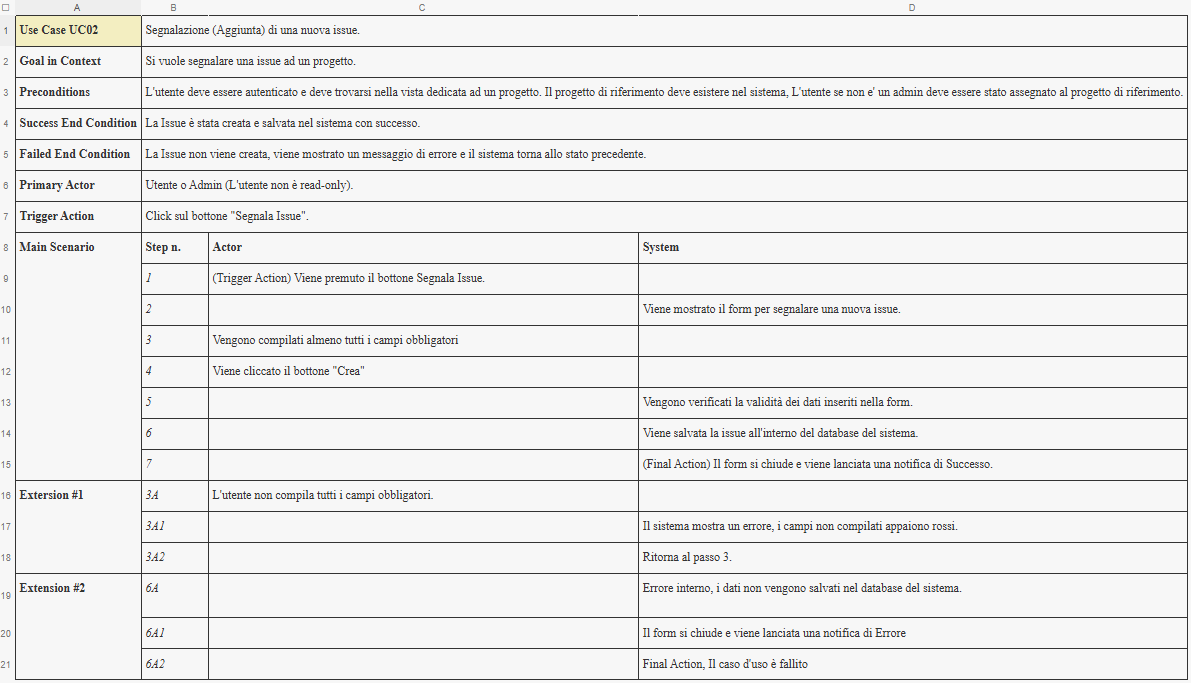
\includegraphics[width=1\linewidth]{./Assets/Chapters/cockburn.png}
	\end{table}

	
	\chapter{Prototipazione via Mockup}
I seguenti \textit{Mockup} rappresentano una simulazione grafica delle principali \textbf{interfacce utente} presenti nel sistema.\\
Hanno lo scopo di mostrare in modo chiaro il \textbf{flusso di navigazione} e le \textbf{funzionalità previste} per gli utenti. Le schermate realizzate permettono di visualizzare il \textbf{comportamento del sistema} e l'\textbf{esperienza d'uso} prima di passare all'implementazione effettiva.

\section{Descrizione dettagliata dei Mockup}
\subsection{Schermata di Login}

\begin{figure}[h]
	\centering
	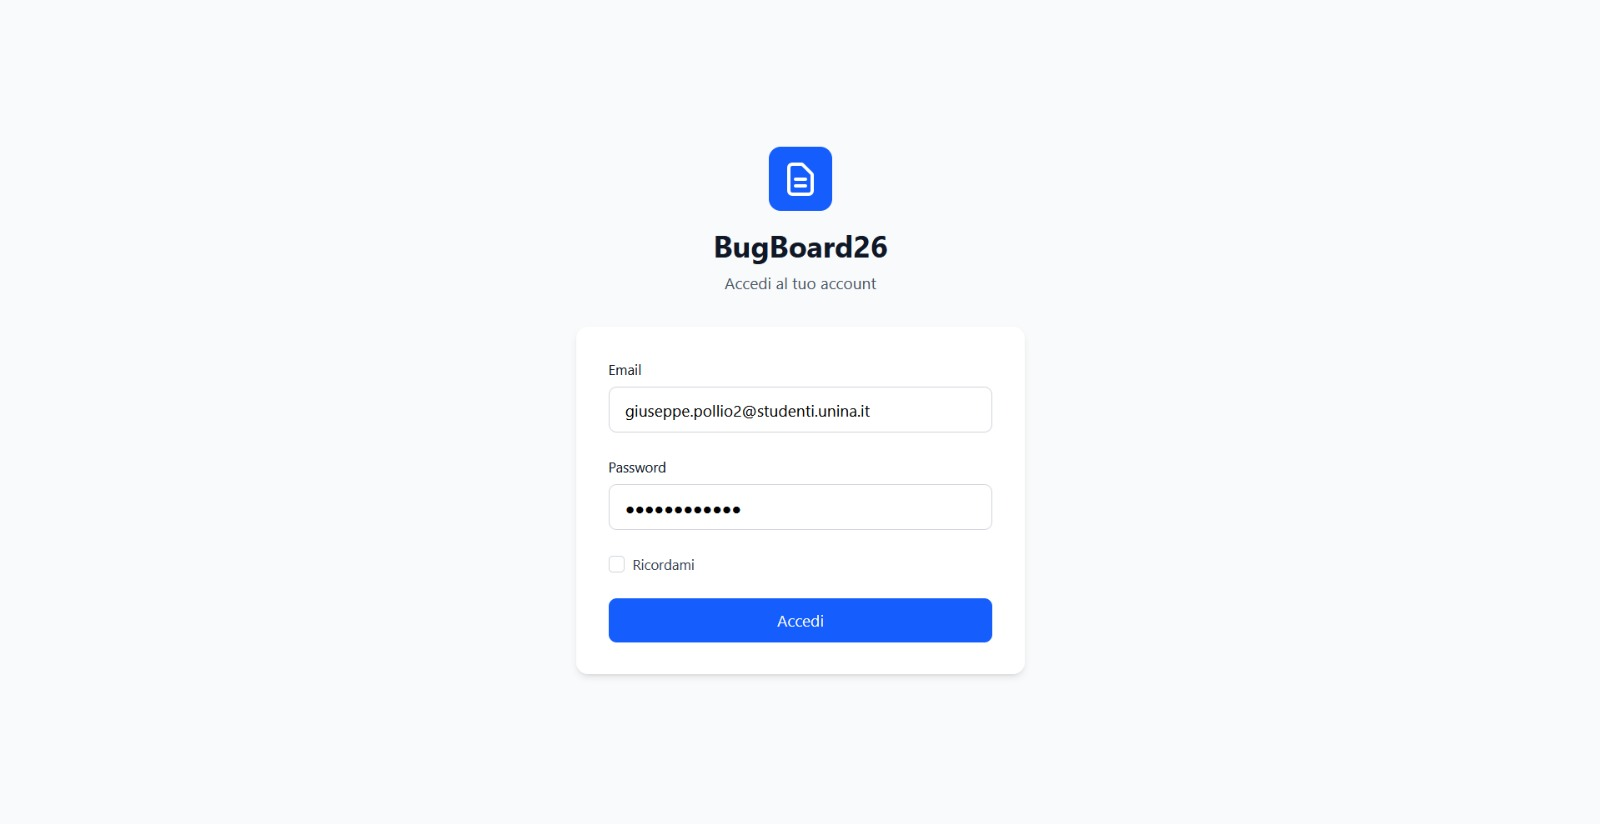
\includegraphics[width=1\linewidth]{./Assets/Chapters/mkp1.jpg}
	\caption{Schermata di login}
\end{figure}

La schermata raffigurata rappresenta la pagina di login al sistema.\\
L'utente da qui inserisce le proprie credenziali per accedere al sistema, scegliendo inoltre se mantenere la sessione attiva tramite la spunta "Ricordami"\\
Una volta autenticato, viene reindirizzato all'\textit{Area progetti}

\subsection{Area progetti}

\begin{figure}
	\centering
	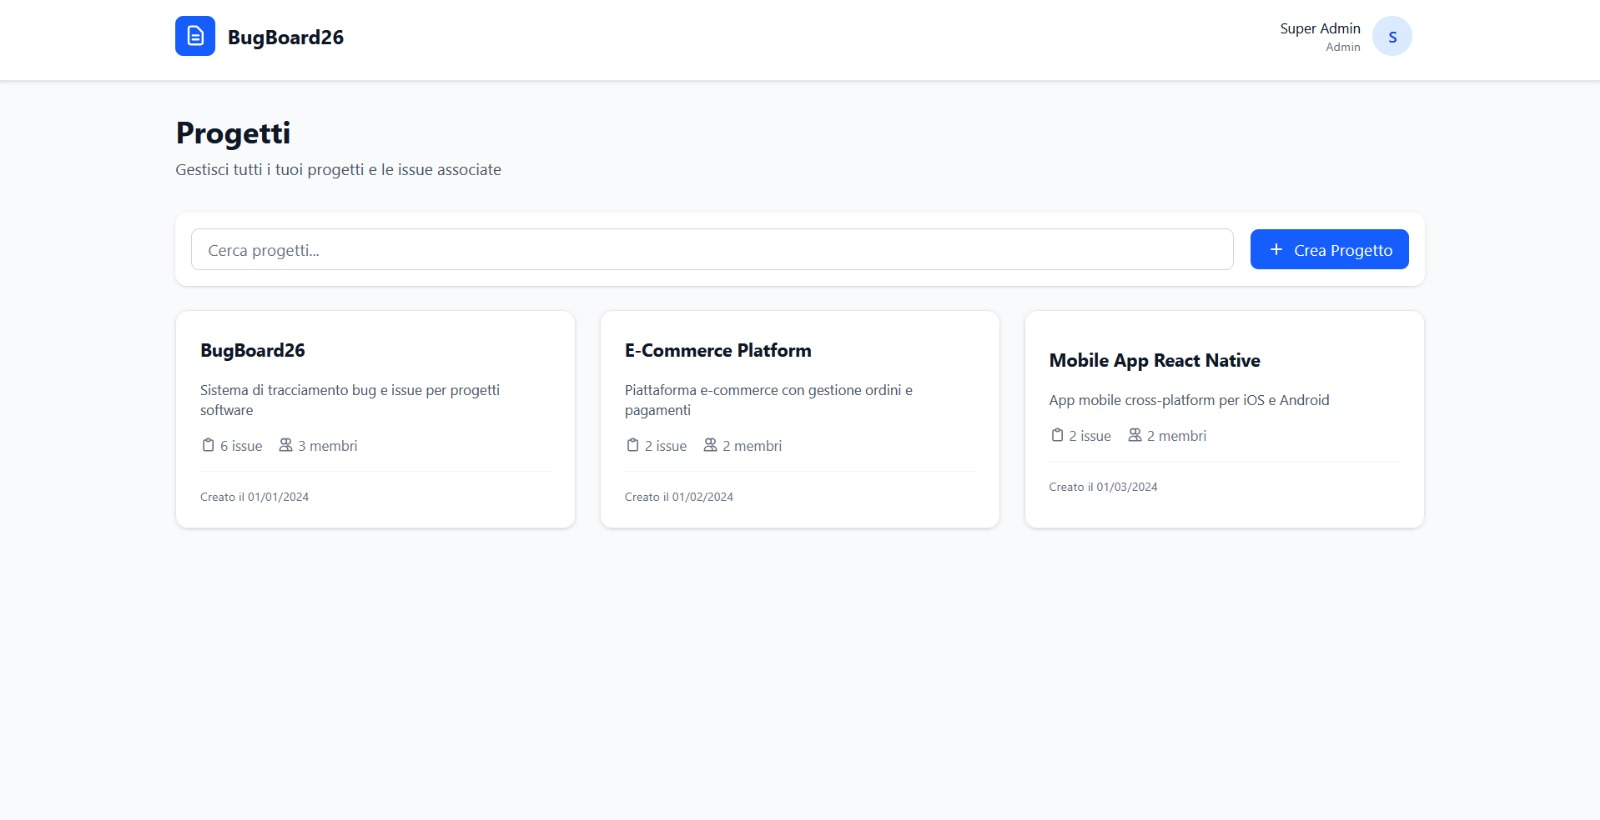
\includegraphics[width=1\linewidth]{./Assets/Chapters/mkp2.jpg}
	\caption{Area progetti}
\end{figure}
Una volta effettuato il login, l'utente accede all'area dei progetti, dove può visualizzare i progetti a cui partecipa.\\
In alto è presente una barra di ricerca per cercare i progetti e un pulsante per crearne di nuovi (visibile solo con account Admin)\\
Ogni progetto è caratterizzato da:
\begin{itemize}
	\item Nome del progetto
	\item Breve descrizione
	\item Numero di \textit{Issue} aperte
	\item Numero di membri del team
	\item Data di creazione
	
\end{itemize}

\subsection{Pagina issues del Progetto}
\begin{figure}
	\centering
	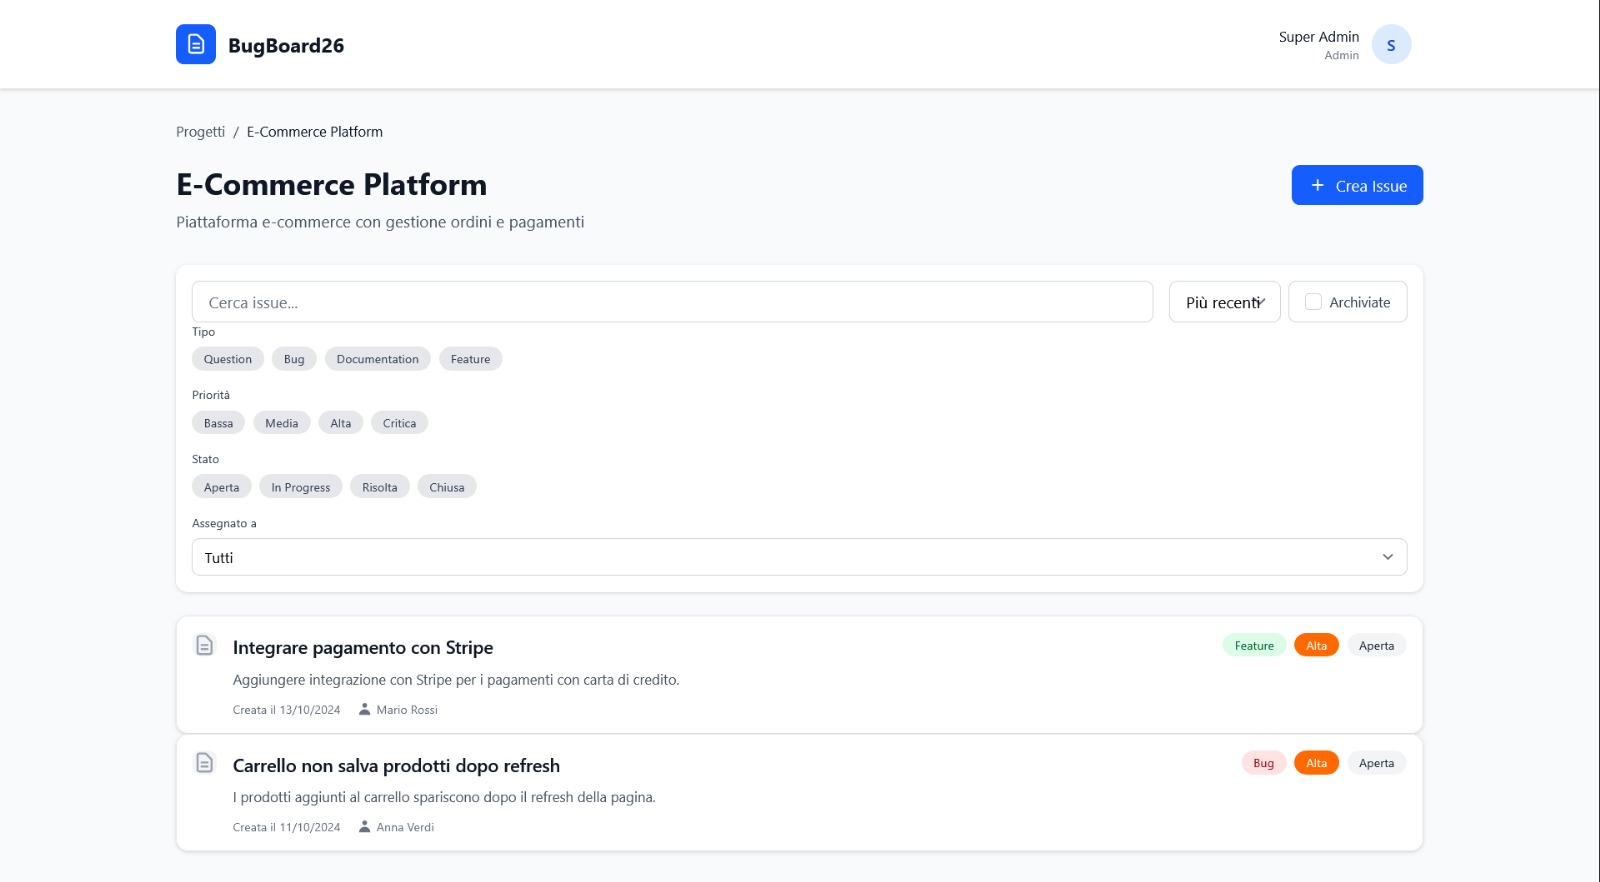
\includegraphics[width=1\linewidth]{./Assets/Chapters/mkp3.jpg}
	\caption{Pagina Issue}s
\end{figure}
Una volta selezionato un progetto, l'utente accede alla pagina delle issues associate.\\
in questa pagina sono visibili tutte le segnalazioni relative al progetto selezionato, con titolo, descrizione, tipo, priorità, stato e autore.\\
Sopra la lista l'utente può filtrare le issues, cercarle nell'apposita barra di ricerca o ordinarle in base alla data di creazione. Inoltre è presente una spunta per visualizzare le issues archiviate.\\
Inoltre è presente il tasto "Crea Issue", che apre il modulo di creazione.


\subsection{Modulo creazione Issue}
\begin{figure}
	\centering
	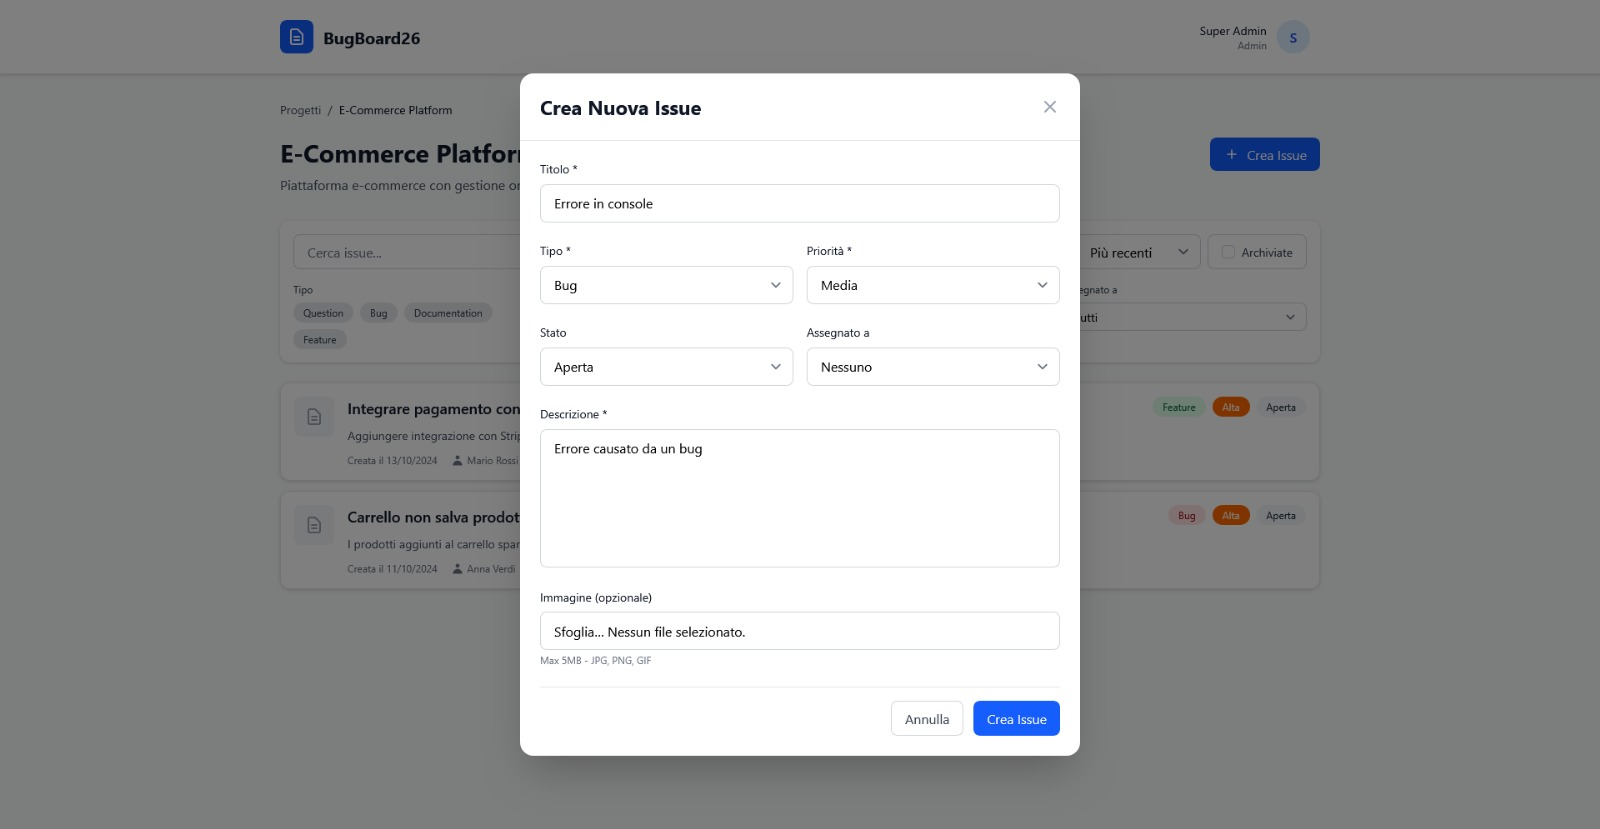
\includegraphics[width=1\linewidth]{./Assets/Chapters/mkp4.jpg}
	\caption{Creazione Issue}
\end{figure}
Il \textit{mockup} sopra mostra il form di inserimento di una nuova \textit{issue}.\\
L'utente deve compilare alcuni campi obbligatori (titolo, tipo, priorità, descrizione), ma può anche aggiungerne di facoltativi (immagine, stato, assegnatario).\\
In fondo al modulo, sono presenti i pulsanti "Annulla" e "Crea Issue", che permettono rispettivamente di chiudere la schermata o di confermare la segnalazione.

\subsection{Aggiornamento lista Issue}
\begin{figure}
	\centering
	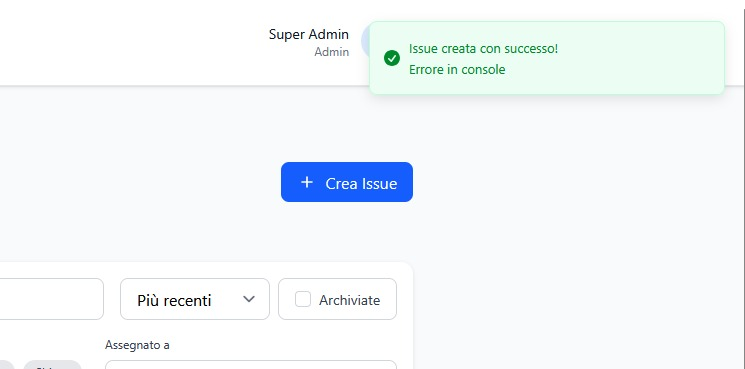
\includegraphics[width=1\linewidth]{./Assets/Chapters/mkp5.jpg}
	\caption{Aggiornamento lista}
\end{figure}
Il \textit{mockup} raffigura la schermata aggiornata dopo la creazione di una nuova \textit{issue}. La lista \textit{issues} viene aggiornata automaticamente con la nuova voce in elenco.\\
Il sistema mostra inoltre una notifica di \textit{feeback} in alto sullo schermo che conferma l'operazione di aggiunta (o segnala un eventuale errore se non è stato possibile aggiungere l'\textit{issue})

\subsection{Errore durante la compilazione del modulo (creazione issue)}
\begin{figure}
	\centering
	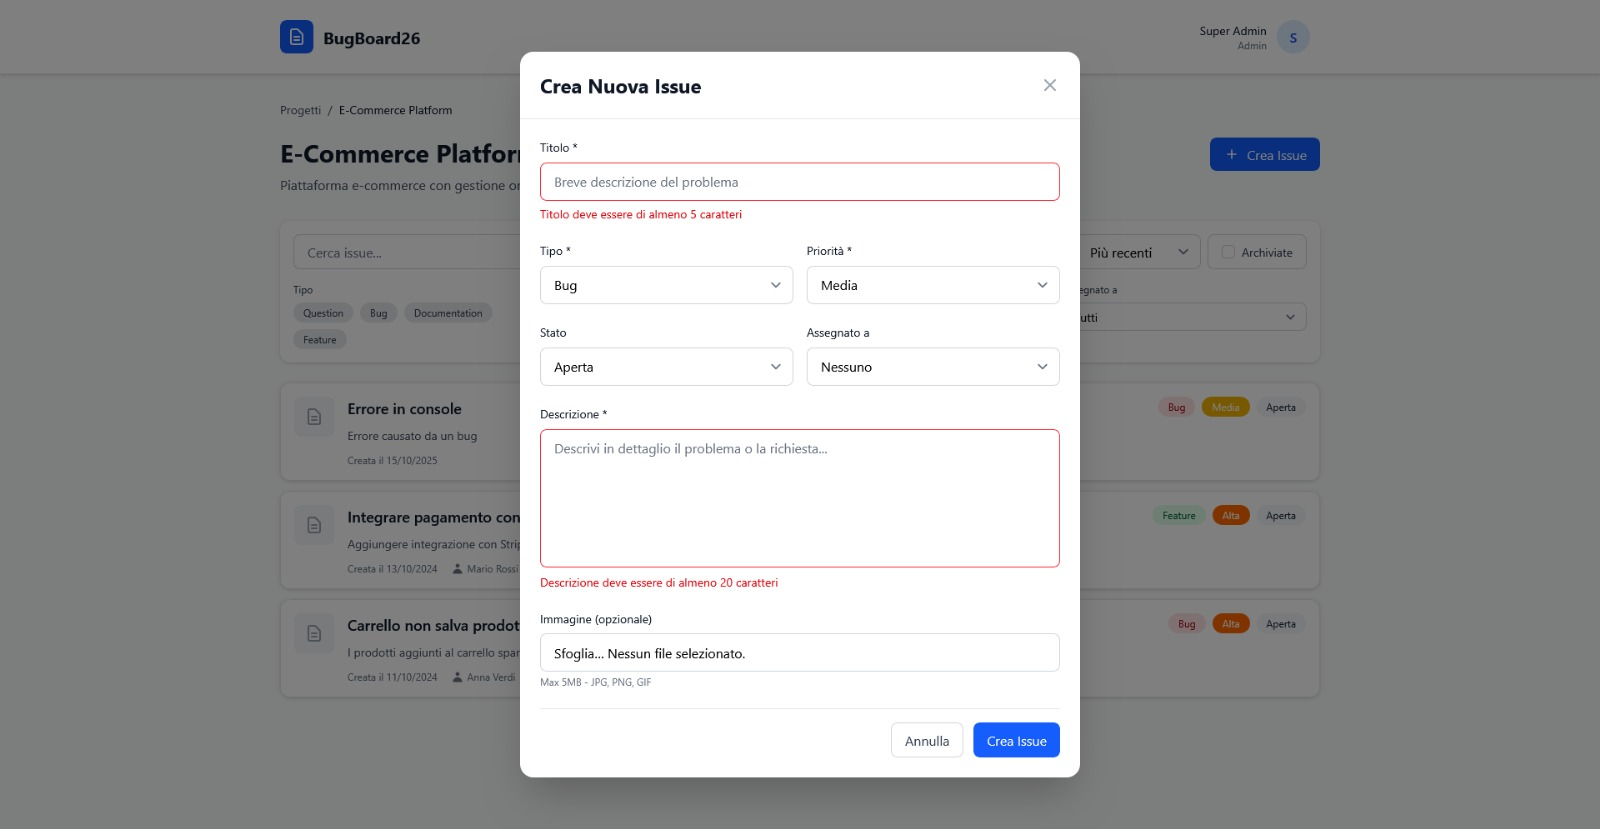
\includegraphics[width=1\linewidth]{./Assets/Chapters/mkp6.jpg}
	\caption{Errore 1}
\end{figure}
Durante la compilazione del modulo, se ci si dimentica di inserire tutti i campi obbligatori, si riscontra il seguente errore. Vengono mostrate i vari messaggi di errore e il sistema aspetta che l'utente corregga l'inserimento dei campi per continuare.

\subsection{Errore interno, per qualche motivo i dati non vengono salvati nel database}
\begin{figure}
	\centering
	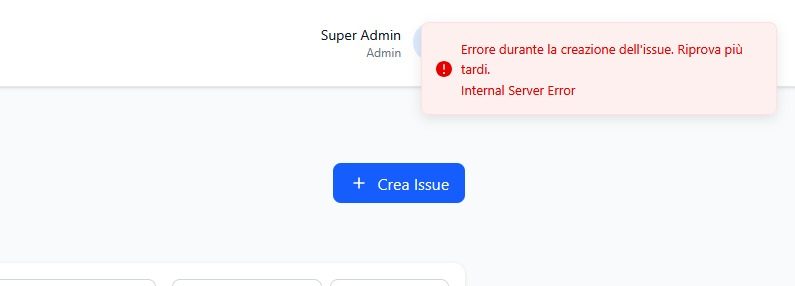
\includegraphics[width=1\linewidth]{./Assets/Chapters/mkp7.jpg}
	\caption{Errore 2}
\end{figure}
Una volta finita la compilazione del modulo, dopo aver premuto il tasto "Crea", se il sistema cade in un qualsiasi errore interno allora viene lanciato il seguente messaggio di errore nella forma di una notifica.

	
\end{document}